\section{\acf{CPS}}
A \acf{CPS} is a network of distributed controllers that manage the physical processes of the system~\cite{cps-design}~\cite{alur2015principles}. 
\ac{CPS} encompass a wide variety of disciplines, from mechatronics to civil infrastructure, illustrated in Figure~\ref{fig:cps}.
\ac{CPS} operate in the physical world, where environments can be unpredictable and uncontrolled.
This introduces safety concerns for the \ac{CPS}; the hardware must be predictable and reliable and the software must be predictable and reliable.
This thesis focuses on the software requirements for \ac{CPS}.

\begin{figure}[H]
	\centering
	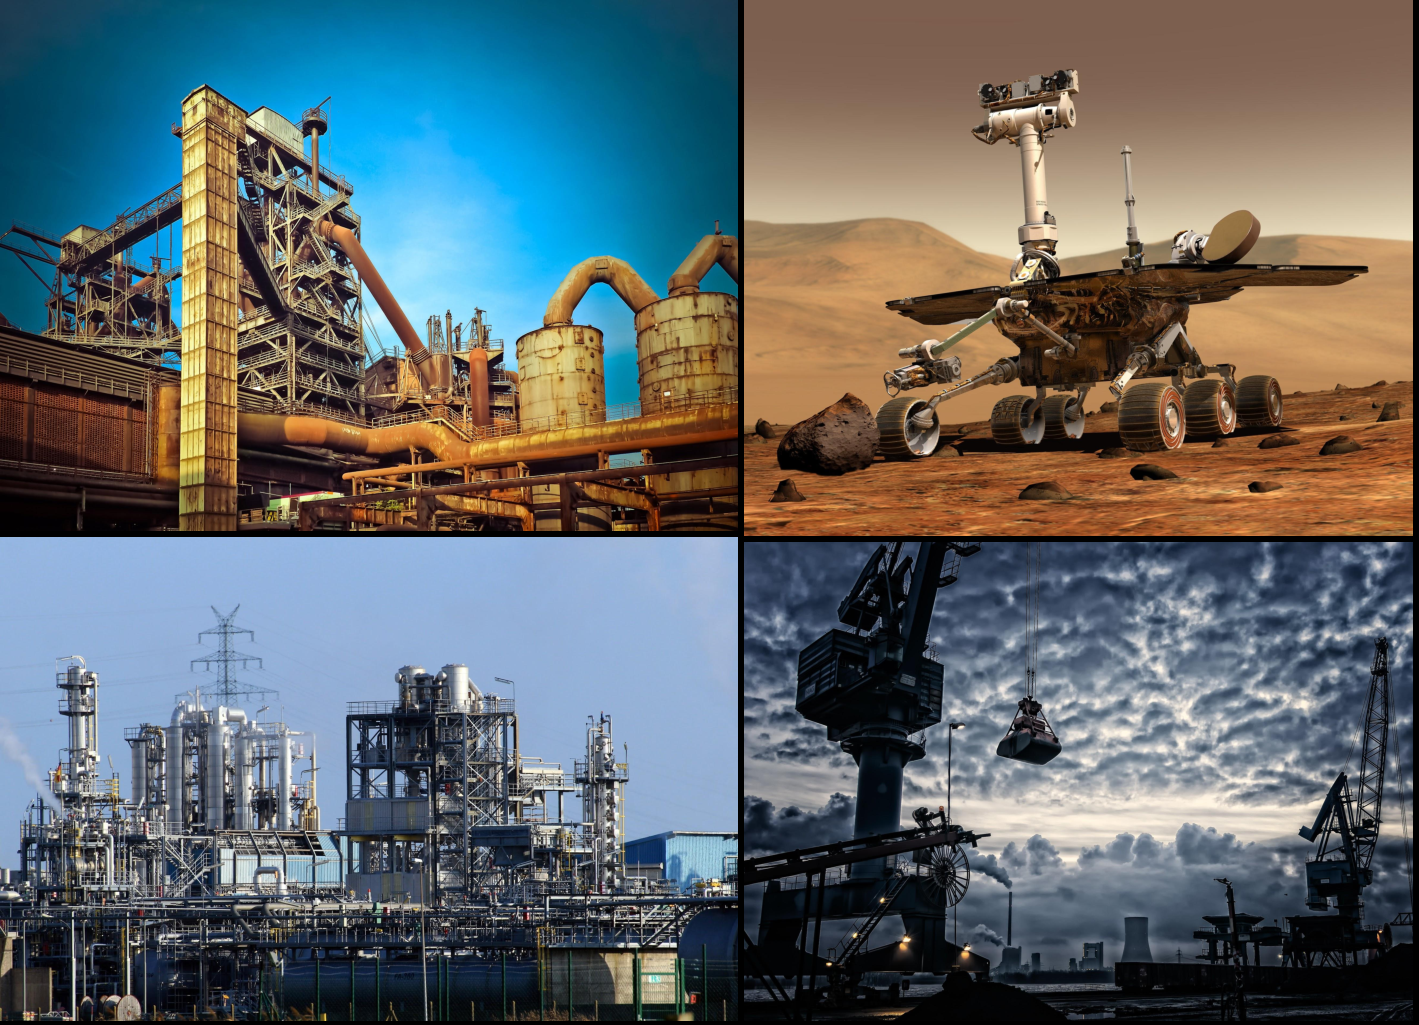
\includegraphics[width=\textwidth]{Content/fig/1234.pdf}
	\caption{Examples of \ac{CPS}~\cite{industry-pic}~\cite{crane-pic}~\cite{rover-pic}~\cite{factory-pic} \label{fig:cps}}
\end{figure}

\ac{CPS} applications encompass real-time systems, where the system needs to satisfy a set of timing requirements to ensure correct operation. 
Here, a missed deadline may result in catastrophic consequences, making these \ac{CPS} highly \textit{safety-critical}. 
These have strict timing and functionality requirements --- any errors in control can result in physical damage, injuries, and/or fatalities~\cite{ANNDevModel1999}. 


\section{\acf{AI} and \acf{ML}}
\acf{ML} is a field of data science where \acf{AI} are taught to learn large and/or complex data relationships~\cite{ai}.
\ac{AI} come in many shapes and forms, from decision trees to \acfp{ANN}~\cite{ai-types}.
\ac{AI} were invented to fill a gap that humans cannot, where they can store a huge number of data relationships and learn new relationships where a person would struggle.
\ac{AI} are used all over industry, from industrial systems, so cybernetics and robotics (such as Figure~\ref{fig:ai-girl}).

\begin{figure}[H]
	\centering
	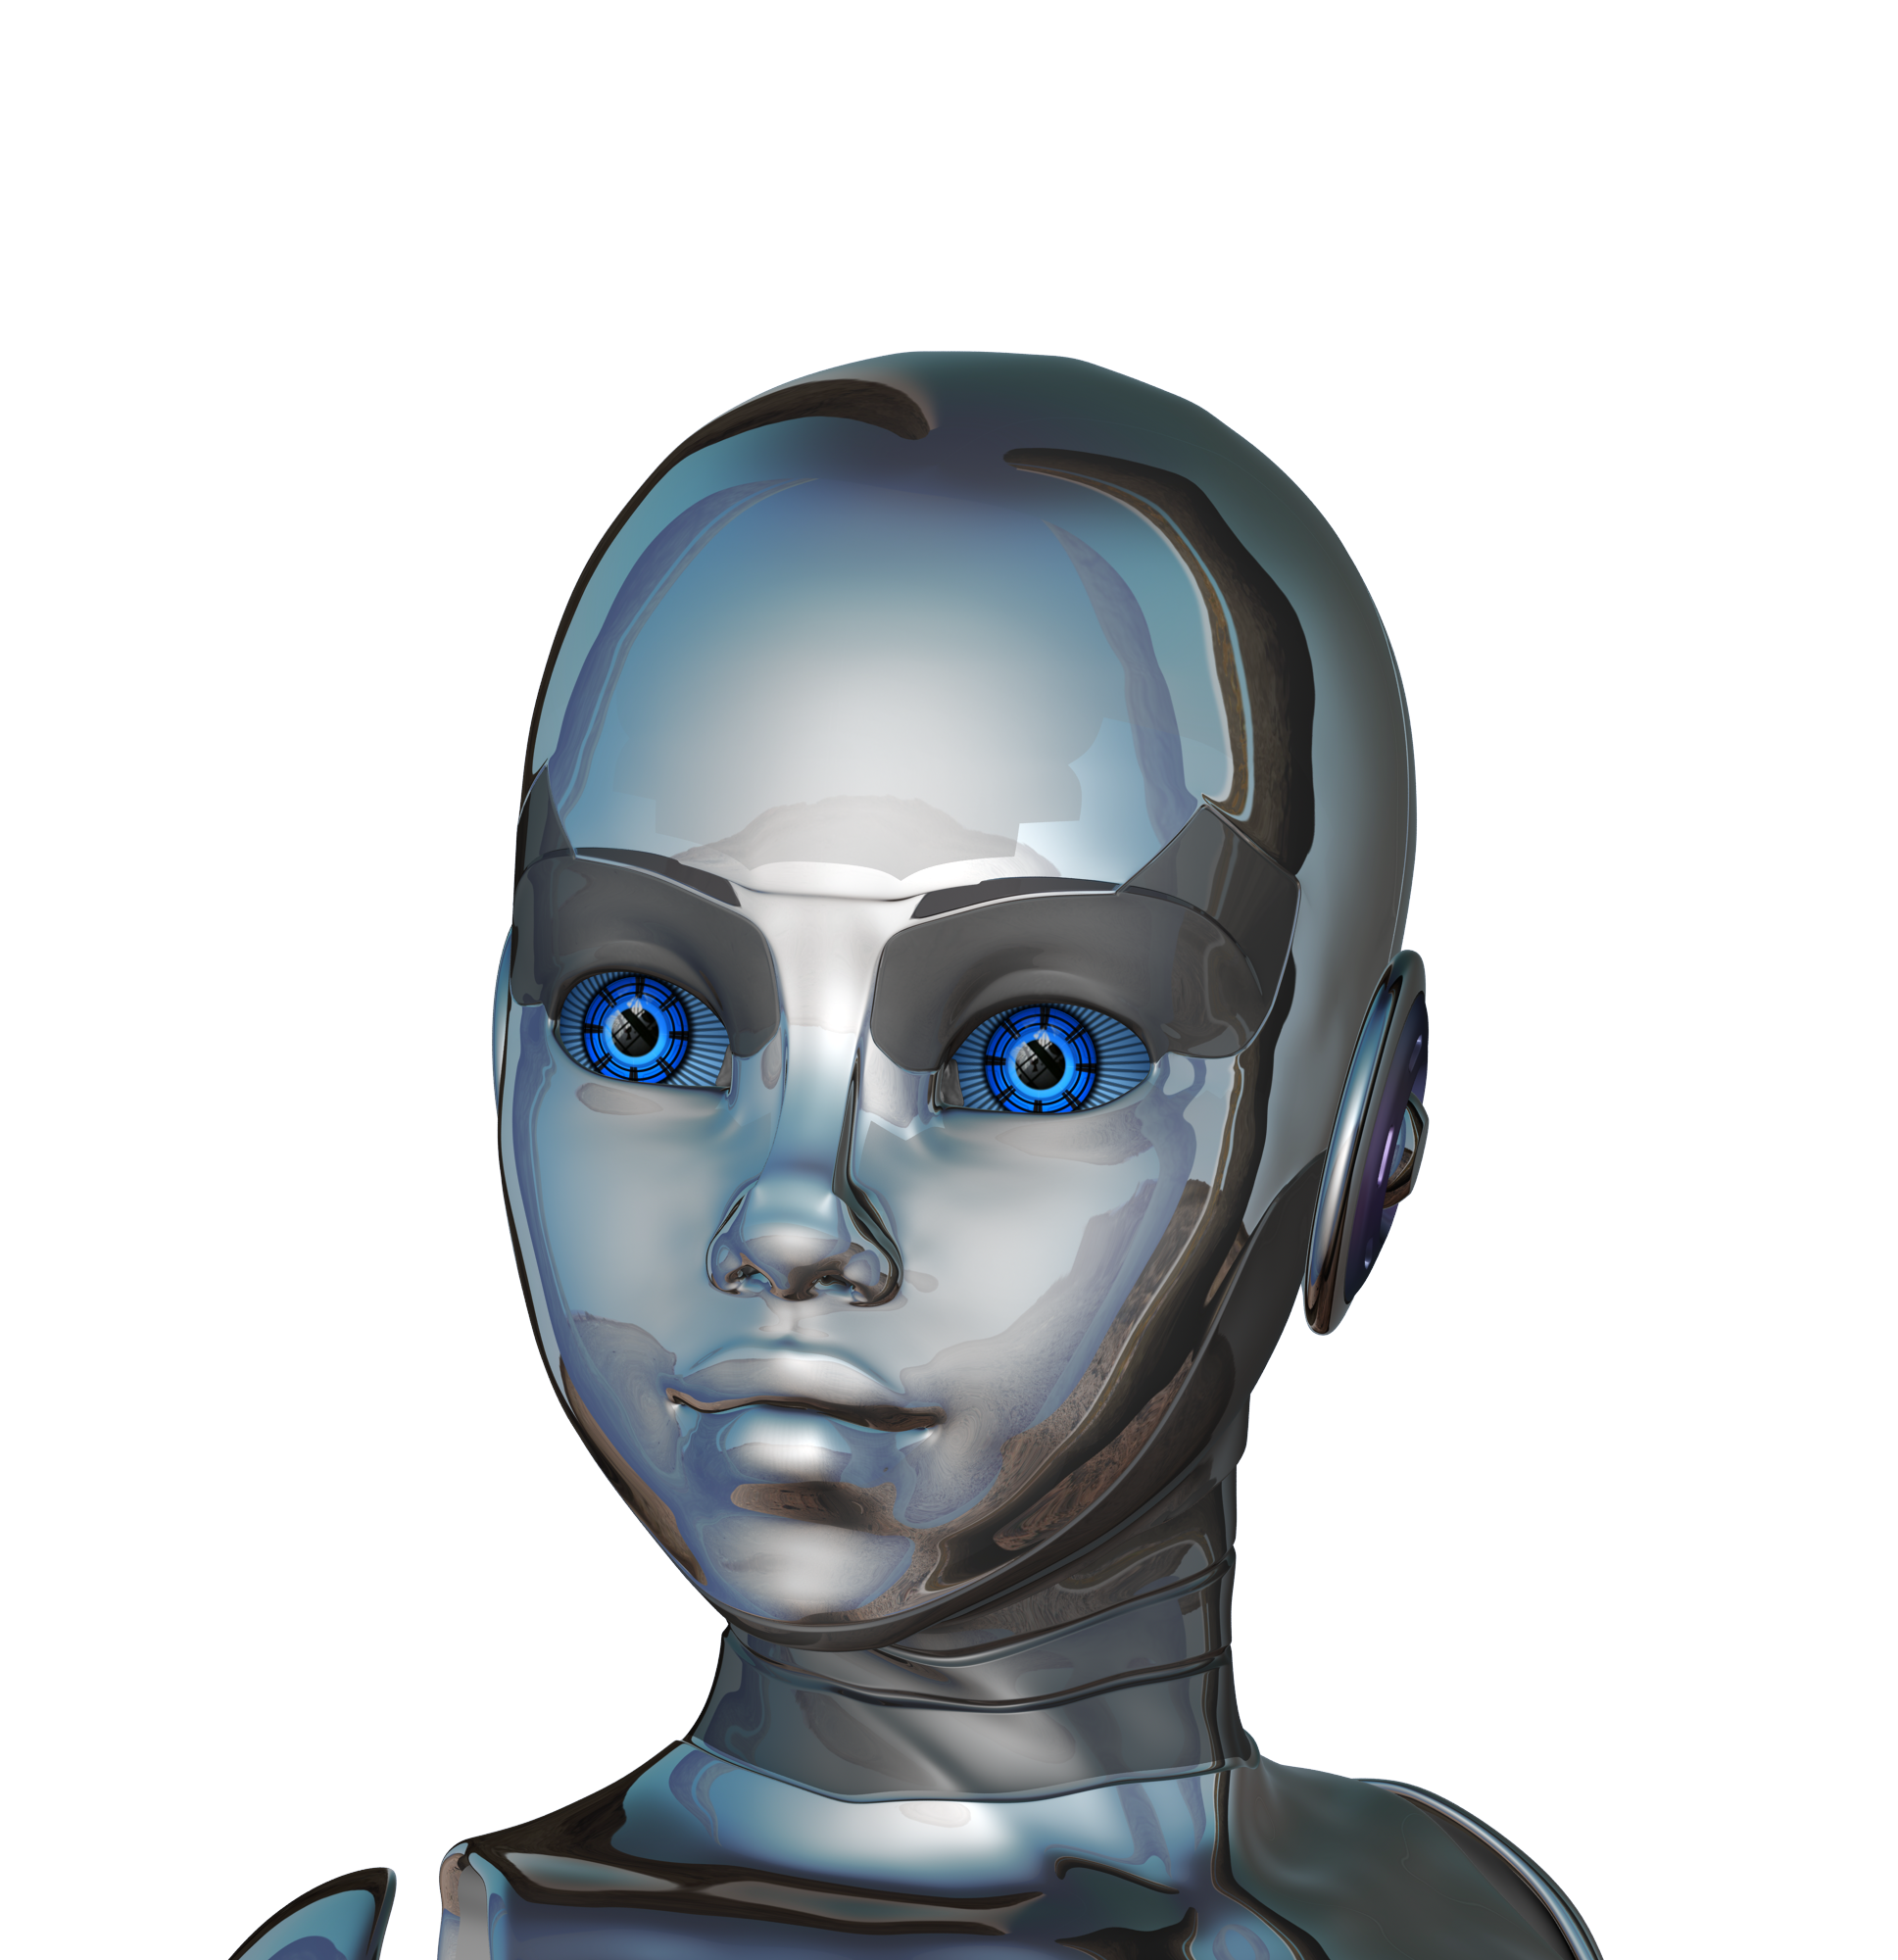
\includegraphics[width=0.4\textwidth]{Content/fig/ai-girl.png}
	\caption{Robotics are a common source of \ac{AI}~\cite{robotgirl-pic} \label{fig:ai-girl}}
\end{figure}

\ac{AI} are increasingly used in \ac{CPS}, where safety is critical.
However, the nature of \ac{AI} is non-linear, leaving many \ac{AI} hard to verify and validate.
Additionally, as \ac{AI} adapt to learn larger data sets and more complex relationships, the size and complex of the \acp{AI} increase.
Some of these \ac{AI} are susceptible to verification and validation techniques, however, as they grow in size, these techniques take longer and more resources to implement.
In \ac{CPS}, it is essential for all components to be verified and validated, and thus the issue with \ac{AI} in \ac{CPS} is made clear.

\subsection{\acfp{ANN}}
\acp{ANN} are a type of \ac{AI} designed to model the human brain~\cite{kohonen1988introduction}.
The resulting \ac{AI} are generally large and complex.
They are composed of interconnected artificial neurons, each passing messages along to the next, and can be represented mathematically by a long, non-linear equation.
They are able to store large and complex data relationships, like their biological counterpart.
The result of this is that \acp{ANN} are extremely difficult to verify or validate.

\acp{ANN} are often used in big data, but also show up in \ac{CPS} such as \acfp{AV}.
Their use in \ac{CPS} is highly contended, as \acp{ANN} are not 100\% reliable and accidents happen~\cite{coldewey_2018}.
Thus, it is of utmost importance that any \ac{ANN} used in any \ac{CPS} is able to verified to be safe for that system in \textit{any} environment.
Without that guarantee of safety, the use of \ac{AI} in such systems is risky.
There exists a large body of research towards the safety of \acp{ANN}, but there are still opportunities for new approaches to safe \acp{ANN} to emerge.

\subsection{\acf{WCET}}
\todo{Section on timing analysis techniques}

\section{Contribution}
This thesis provides novel techniques to the verification and validation of \acfp{ANN} in \acf{CPS}.
There is a large body of work regarding the safety of \acp{ANN}, ranging across a whole variety of applications and approaches.
However, no work has been done regarding the synchronous implementation of \acp{ANN} and the verification available to synchronous \acp{ANN}.  
This thesis addresses the issue of safe \acp{ANN} using synchronous semantics.

In this thesis, a new \ac{ANN} library was created to look at the benefits of synchronous \acp{ANN}.
In some of the benchmarks, an existing library called Darknet~\cite{darknet13} was used to implement some of the more complex \acp{ANN}.
However, a tool chain was created to replace Darknet that compiles Keras~\cite{chollet2015keras} \acp{ANN} to the created \ac{ANN} library.

The major contributions of this thesis are as follows:
\begin{itemize}
	\item A time predictable approach to \acp{ANN} is developed using the synchronous language Esterel~\cite{berry2000foundations}. These predictable \acp{ANN} are termed \acfp{SNN} and are defined using formal methods. Using T-CREST as a platform, timing of these \acp{SNN} was done. These \acp{SNN} provide a safe approach to implementing \acp{ANN} in \ac{CPS}. The results of the \acp{SNN} are presented using a set of benchmarks. 
	\item \acfp{MNN} are proposed as a framework for the composition of multiple \acp{SNN}. The thesis provides formal definitions for the \acp{MNN} and benchmarks are presented that show their efficacy. 
	\item The thesis proposes the \acf{RV} of \acp{MNN} as an approach to dealing with input perturbation of \acp{ANN} that have complex inputs, such as image classification \acfp{CNN}. An \acf{AV} case study is created for this work, with an \ac{AV} object detection simulation created to prove the benefits of this proposition. 
\end{itemize}

\section{Thesis Structure}
Chapter 2 gives a basic understanding of the concepts required to understand this research towards safe \acp{ANN} for \ac{CPS}.

Chapter 3 introduces the concept of \acfp{SNN} and their timing properties.
Formal definitions of \acp{SNN} and their related components are provided in this chapter.
Furthermore, the meta combinations of these \acp{SNN}, termed \acp{MNN}, and the usefulness of such \acp{MNN} in \ac{CPS} is discussed.
Lastly, a new Python tool chain that creates these \acp{SNN} from Keras is also introduced.

Chapter 4 introduces the concept of \acf{RE} in combination with \acp{SNN}. 
This chapter provides formal definitions for the enforcers and safety policies enforced.
An \acf{AV} case study is made for this chapter to show the efficacy of the \ac{RE} of \acp{SNN}.

Chapter 5 proposes two different methods, used in tandem, to increase the safety of systems with complex inputs, such as object detection for \acp{AV}.
The first method is the use of \acp{MNN} to increase the classification accuracy of \acp{SNN}.
The second expands on Chapter 4, and introduces the use of \ac{RV} to increase the safety of system where \ac{RE} cannot do so.
An \ac{AV} object detection simulation is created as a complex \ac{MNN} 

Finally, conclusions are drawn on the synchronous approach proposed in this thesis to creating safe \acp{ANN}.

